\documentclass[10pt]{article}
\usepackage[utf8]{inputenc}
\usepackage[spanish]{babel}
\usepackage[usenames,dvipsnames,svgnames,table]{xcolor}
\usepackage{multirow}
\usepackage{diagbox}
\usepackage{booktabs}
\usepackage{anysize} 
\usepackage{hyperref}
\usepackage{helvet}
\renewcommand\refname{Referencias}
\marginsize{2cm}{2cm}{2.0cm}{2cm}
\usepackage{enumitem}
\usepackage{setspace}
\usepackage{scrextend}
\addtokomafont{labelinglabel}{\sffamily}

%% Graphics
\usepackage{graphicx}
\usepackage{color}
\usepackage{gensymb}
\usepackage{multirow}
\usepackage{caption}
\usepackage{float}


\hypersetup{
	colorlinks=true,
	linkcolor=blue,
	filecolor=magenta,
	urlcolor=cyan,
	citecolor=blue
}





\begin{document}
	\title{Fundamentos de Bases de Datos \\
		Practica 3\\ Modelado de Datos
	} 
	\author{}
	\date{12 de Marzo del 2019}
	\maketitle
	
	\section{Diagrama E/R del caso de uso}
	
	El siguiente diagrama esta basado de acuerdo a las especificaciones en el caso de uso.
	
	\begin{figure}[H]
		\centering
		%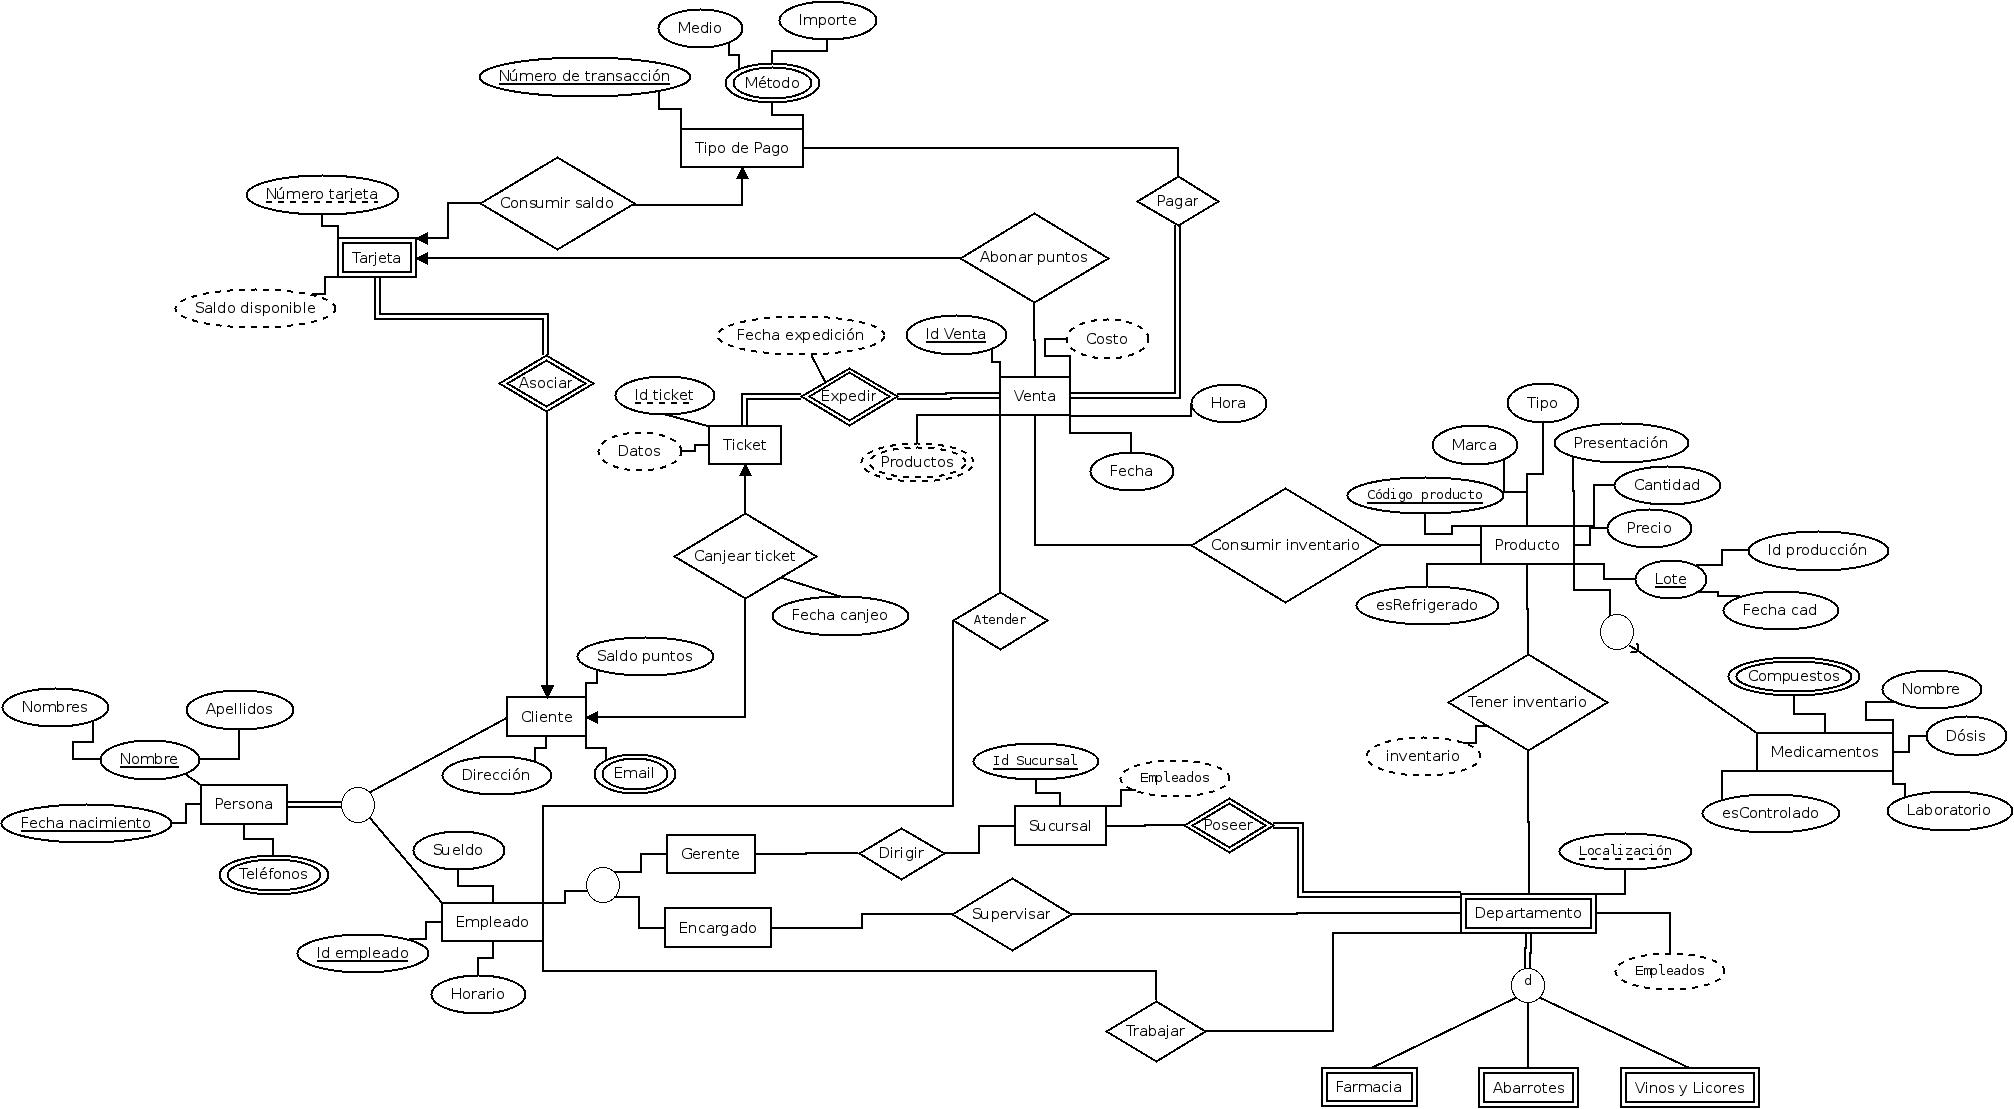
\includegraphics[width=1 \textwidth]{practica03.jpeg}
		\caption{Diagrama E-R para "\,El rey de los Abarrotes ".}
	\end{figure}
	
	
	\section{Desarrollo}
	Se decidió modelar el caso de uso de la siguiente manera.
	\subsection{Entidades}
	\begin{itemize}
		\item Fuertes
		\begin{description}[leftmargin=8em,style=nextline]
			\item [Sucursal] Esta entidad es necesaria porque que las demás 
			entidades tengan sentido. Tiene como atributos 
			\textit{Número de sucursal, Nombre de sucursal, Dirección}\\
			\item [Persona] Se decidio poner una entidad persona porque un 
			empleado también puede ser cliente de la tienda y tener asociada una 
			tarjeta. Tiene como atributos \textit{Nombre, Dirección, Telefono,}\\
			\item [Empleado:] Es una entidad que se deriva de persona y 
			corresponde a las personas que trabajan en alguna sucursal.\\
			\item [Gerente] Es un empleado que supervisa una sucursal. Se usa 
			para llevar la cuenta de quien supervisa que lugares.\\
			\item [Encargado] Es un empleado que supervisa un departamento. 
			Se usa para llevar la cuenta de quien supervisa que lugares.\\
			\item [Cliente] Esta entidad se deriva de persona. Se usa para 
			llevar registro de los datos de los clientes. Notemos que como el 
			saldo es independiente de la tarjeta (pues esta se puede perder) el 
			saldo se guarga en los atributos del cliente.\\
			\item [Venta] En una entidad asociativa que representa la venta de 
			un producto, ya que esta requiere de mucha información de varias 
			entidades.\\
			\item [Ticket] Esta entidad es necesaria porque contiene la 
			información sobre la venta que se realizo, el tipo de artículos que 
			el cliente adquirió, el empleado que efectuo la venta, el numero de 
			sucursal donde se hizo la compra, la forma de pago.\\
			\item [Producto] Modela un ejemplar especifico de un producto, para 
			llevar bien registros de los lotes y las ventas.\\
			\item [Tipo de pago:] Esta entidad indica el tipo de pago que 
			realiza un cliente. Entidad que sirve como catalogo al no poder 
			restringir dominios en el modelo E/R.\\
			\item [Medicamentos] Es una especialización de producto, pues para 
			estos sse requiere guardar información extra.
			
			
		\end{description}
		\item Débiles
		\begin{description}[leftmargin=8em,style=nextline]
			\item [Tarjeta:] Corresponde a la tarjeta digital de puntos y es 
			una entidad débil porque debe estar asociado a un cliente.\\
			\item [Departamento] Modela los departamentos de una sucursal. Es 
			débil porque todo departamento pertenece a una sucursal.\\
			\item [Abarrotes] Especialización de departamento, encargada de 
			abarrotes.\\
			\item [Vinos y Licores] Especialización de departamento, encargada de 
			vinos y licores.\\
			\item [Farmacia] Especialización de departamento, encargada de 
			medicamentos.
		\end{description}
	\end{itemize}
	
	\subsection{Relaciones}
	\begin{itemize}
		\item
		
		\begin{description}[leftmargin=9em,style=nextline]
			\item[Trabajar] Esta relación esta asociada con la entidad empleado 
			y departamento, ya que la entidad departamento contiene la 
			información de la sucursal podemos saber en que sucursal trabaja 
			esa persona.\\
			\item[Supervisar] Relación que indica que supervisor está a cargo de 
			que departamento. \\
			\item[Dirigir] Indica que gerente está a cargo de que sucursal. \\
			\item[Pagar] Esta relación se asocia con la entidad tipo de pago y 
			venta, ya que el cliente puede pagar de diferentes formas, en 
			efectivo, tarjeta de credito o debito o con su tarjeta digital 
			de puntos.\\
			\item[Abonar puntos] Esta relación esta asociada con la entidad 
			venta y tarjeta, ya que al efectuarse una compra y si el cliente 
			presenta su tarjeta se le abonan los puntos correspondientes.\\
			\item[Expedir] Esta relación esta asociada con la entidad venta y 
			ticket porque en cada venta que se haga se deberá generar un ticket,
			además de que tiene el atributo  \textit{fecha de expedición} porque
			será importante para que el cliente pueda abonar los puntos 
			generados si al momento de efectuar su compra no presenta su tarjeta
			lo podrá hacer después con su ticket.\\
			\item[Atender] Relación que indica que empleado atendió que venta.\\
			\item[Canjear ticket] Esta relación esta asociada con la entidad 
			cliente y ticket, tiene como atributo \textit{fecha de canjeo}, 
			esta operación tiene una fecha limite y si no cumple con lo 
			establecido no se le podrá abonar los puntos al cliente.\\
			\item[Consumir saldo] Es una relación entre la tarjeta y el tipo de
			pago. Es así pues sólo se debe consumir saldo cuando el cliente elija 
			usar los puntos como medio de pago.\\
			\item[Tener inventario] Indica que un ejemplar de un producto está 
			en el inventario de un departamento. \\
			\item[Consumir inventario] Indica que un ejemplar de un producto 
			fue vendido en una venta específica. \\
			\item[Asociar] Es una relación de pertenencia que asocia a un 
			cliente con una tarjeta. \\
			\item[Poseer] Es una realción de pertenencia que asocia a cada 
			departamento con una sucursal. 
		\end{description}
	\end{itemize}
	
	
	
	
	\section{Bitácora}
	
	\begin{labeling}{alligator}
		\item [04/03] Inicio de proyecto Categorizamos entidades (a-atributadas)
		 y relaciones sin detalles ($\#$, part, ...). PENDIENTES: definir como 
		 representar herencia sin herencia, todo lo que falto en el modelo 
		 (detalles).
		\item [05/03] E-R Ext es válido, adecuamos ejemplos en el laboratorio. 
		\item [07/03] Definir relaciones finales, terminar diseño 'tipo de pago'.
		\item [11/03] La idea esta completa!
	\end{labeling}
	
	
	
\end{document}